\documentclass[border=10pt]{standalone}
\usepackage{tikz}
\usetikzlibrary{shapes, arrows.meta, positioning, shadows}

\begin{document}

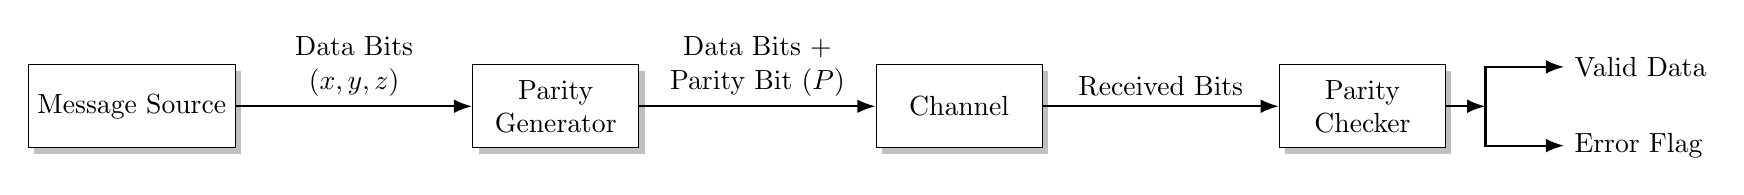
\begin{tikzpicture}[
    auto,
    node distance = 3cm,
    block/.style = {draw, rectangle, minimum height=3em, minimum width=6em, align=center, fill=white, drop shadow},
    sum/.style = {draw, circle, node distance=1cm},
    input/.style = {coordinate},
    output/.style = {coordinate},
    line/.style = {-Latex, thick}
]

    % Nodes
    \node [block] (source) {Message Source};
    \node [block, right=of source] (encoder) {Parity\\Generator};
    \node [block, right=of encoder] (channel) {Channel};
    \node [block, right=of channel] (decoder) {Parity\\Checker};
    \node [coordinate, right=of decoder] (sink) {};
    % Edges
    \draw [line] (source) -- node [midway, align=center] {Data Bits\\($x,y,z$)} (encoder);
    \draw [line] (encoder) -- node [midway, align=center] {Data Bits +\\Parity Bit ($P$)} (channel);
    \draw [line] (channel) -- node [midway, align=center] {Received Bits} (decoder);
    
    % Output edges from decoder
    \draw [line] (decoder.east) -- ++(0.5,0) coordinate (split);
    \draw [line] (split) |- ++(1,0.5) node [right] {Valid Data};
    \draw [line] (split) |- ++(1,-0.5) node [right] {Error Flag};

\end{tikzpicture}

\end{document}
